\newcommand{\A}{\mathbb{A}}
\newcommand{\D}{\mathbb{D}}
\newcommand{\Z}{\mathbb{Z}}
\newcommand{\R}{\mathbb{R}}
\newcommand{\C}{\mathbb{C}}
\newcommand{\T}{\mathbb{T}}
\newcommand{\N}{\mathbb{N}}
\newcommand{\s}{\mathbb{S}}
\newcommand{\tu}{\tilde{U}}
\newcommand{\F}{\mathcal{F}}
\newcommand{\fall}{\;\forall\;}
\newcommand{\exst}{\;\exists\;}
\newcommand{\nexst}{\;\not\exists\;}
\newcommand{\br}{\par\vspace{10pt}}
\newcommand{\Ch}{C_n(X)}
\newcommand{\ch}{C_{n-1}(X)}
\newcommand{\dx}{\Delta_n(X)}
\newcommand{\ddx}{\Delta_{n-1}(X)}
\newcommand{\im}{\text{Im}}
\newcommand{\Ker}{\text{Ker}}

\providecommand{\comm}{\todo[inline, color=SpringGreen!40]}
\providecommand{\duda}{\todo[inline, color=Apricot!40]}

\documentclass{cmat-monografia}

\usepackage{lipsum}
\usepackage{amssymb}
\usepackage{todonotes}
\usepackage[dvipsnames]{xcolor}
\usepackage[figurename=Imagen]{caption}
\usepackage{subcaption}

\theoremstyle{definition}
\newtheorem{df}{Definición}[chapter]
\newtheorem{obs}[df]{Observación}
\newtheorem{ex}[df]{Ejemplo}
\newtheorem{lema}[df]{Lema}

\theoremstyle{remark}
\newtheorem*{dem}{Demostración}

\theoremstyle{plain}
\newtheorem{prop}[df]{Proposición}
\newtheorem{teo}[df]{Teorema}
\newtheorem{cor}[df]{Corolario}


\title{Elementos de la Matemática}

\author{Nicolas Bourbaki}

\subtitle{Topología}

\director{André Weil}

\codirector{Lauren Schwartz}

\inst{ENS}

\coinst{École Polytechnique}

\parindent 0pt


\begin{document}

\maketitle
\begin{abstract}

\vspace{10pt}\par

Un encaje de $S^1$ en $S^2$ es una función $f:S^1\to S^2$ inyectiva y continua. Una función así es un homeomorfismo sobre su imagen, y por lo tanto $f(S^1)$ es una curva cerrada simple $\gamma$. ¿Qué sabemos sobre $\gamma$? Desde hace 150 años se sabe que $\gamma$ separa a $S^2$ en dos componentes conexas. Hace 100 años se probó que además existe un homeomorfismo $h:S^2\to S^2$ que manda $\gamma$ en $S^1$, lo que tiene como consecuencia que las componentes conexas de $\gamma^c$ tienen $\pi_1=0$. \par
\vspace{10pt}
\comm{qué sabemos sobre $ \gamma$ me parece muy general y no sé q cosas más "sabemos" sobre $\gamma$ q se me escapan}

¿Qué pasa en general con encajes de $f:S^{n-1}\to S^n$? Desde hace 100 años sabemos que $f(S^{n-1})^c$ tiene dos componentes conexas. Sin embargo, en estos casos no necesariamente existe un homeomorfismo $h:S^n\to S^n$ que mande $f(S^n)$ al encaje usual de $S^{n-1}\subset S^n$.\br

Estos dos útlimos resultados se probarán en esta monografía. Para el primero se introducirá al lector a la teoría de homología singular y se probarán algunos resultados sobre la misma. Para probar que el homeomorfismo $f$ no necesariamente se extiende a todo $S^n$, darán dos ejemplos de 2-esferas $S$ encajadas en $R^3$ con $\pi_1(S^c)\neq\varnothing$. Además veremos que los $\pi_1(S)$ serán ejemplos de grupos no triviales cuyo abelianizado es trivial.\br

Después veremos cositas de límites inversos y atractores de sistemas dinámicos.\comm{escribir xd}

\end{abstract}

\chapter{Preliminares}

En general, notamos $S^n := \{x\in\R^n : \|x\|=1\}$, y decimos que una $n-$esfera es un espacio topológico $S$ tal que existe un homeomorfismo $h:S\to S^n$.\br

\comm{agregar: grupo libre, notación}

\chapter{Homología simplicial}

En esta sección introduciremos al lector a la teoría de homología simplicial. Se presentarán algunas definiciones y ejemplos con el objetivo de desarrollar primeras intuiciones sobre la teoría de homología, para luego dar paso a la definición de homología singular en el siguiente capítulo. \br 

% El objetivo será probar que una $(n-1)$-esfera separa $\R^n$ en dos componentes conexas, y que estas componentes conexas tienen la misma homología de un punto. \br

Para empezar, definiremos lo que es un $n$-símplice:\br

\begin{df} Un $n$-símplice es el menor conjunto convexo de $\R^{m}\; (m\geq n)$ que contiene $n+1$ puntos $v_0,\dots,v_n$, tales que $v_1-v_0$, $v_2-v_0$, $\dots$, $v_n-v_0$ son linealmente independientes. Llamaremos vértices a estos $v_i$.\end{df}\br

En general, dado un $n$-símplice, vamos a darle un orden a sus vértices, y notaremos al símplice $[v_0,v_1,\dots,v_n]$ de acuerdo con este orden. \br

\begin{df}
Un orden en los vértices nos induce un orden en la restricción a un subconjunto de esos vértices. Haremos uso de la siguiente notación:
$$[v_0,\dots,\hat{v_i},\dots,v_n]:=[v_0,\dots,v_{i-1},v_{i+1},\dots,v_n]$$ \br
Esta es una forma de notar el $(n-1)$-símplice obtenido al sacar $v_i$ del conjunto de vértices de $[v_0,\dots,v_n]$ y tomar el menor conjunto convexo que contiene a los vértices restantes. \br

Diremos que $[v_0,\dots,\hat{v_i},\dots,v_n]$ es una cara de $[v_0,\dots,v_n]$.\br

\begin{obs}
El borde de un $n$-símplice $\Delta^n$ es la unión de sus $n+1$ caras, lo notaremos $\partial\Delta^n$. \br
\end{obs}

Llamaremos aristas a los $2$-símplices con vértices $v_i, v_j\in\{v_0,\dots,v_n\}$. Estas también heredan el orden de $[v_0,\dots,v_n]$, y por lo tanto las notamos $[v_i,v_j]$ si $i<j$.\br
\end{df}

% Al definirlo así, implícitamente le estamos dando a los vértices de $[v_0,\dots,\hat{v_i},\dots,v_n]$ el orden heredado de restringir el orden de $[v_0,\dots,v_n]$ al nuevo conjunto de vértices. \br

Como se muestra en la imagen \ref{simplices}, un ejemplo de $3$-símplice es un tetraedro en $\R^3$, un $2$-símplice es un triángulo en $\R^2$, un $1$-símplice es un intervalo en $\R$, y un $0$-símplice es un punto.\br


\begin{figure}[h!]
    \centering
    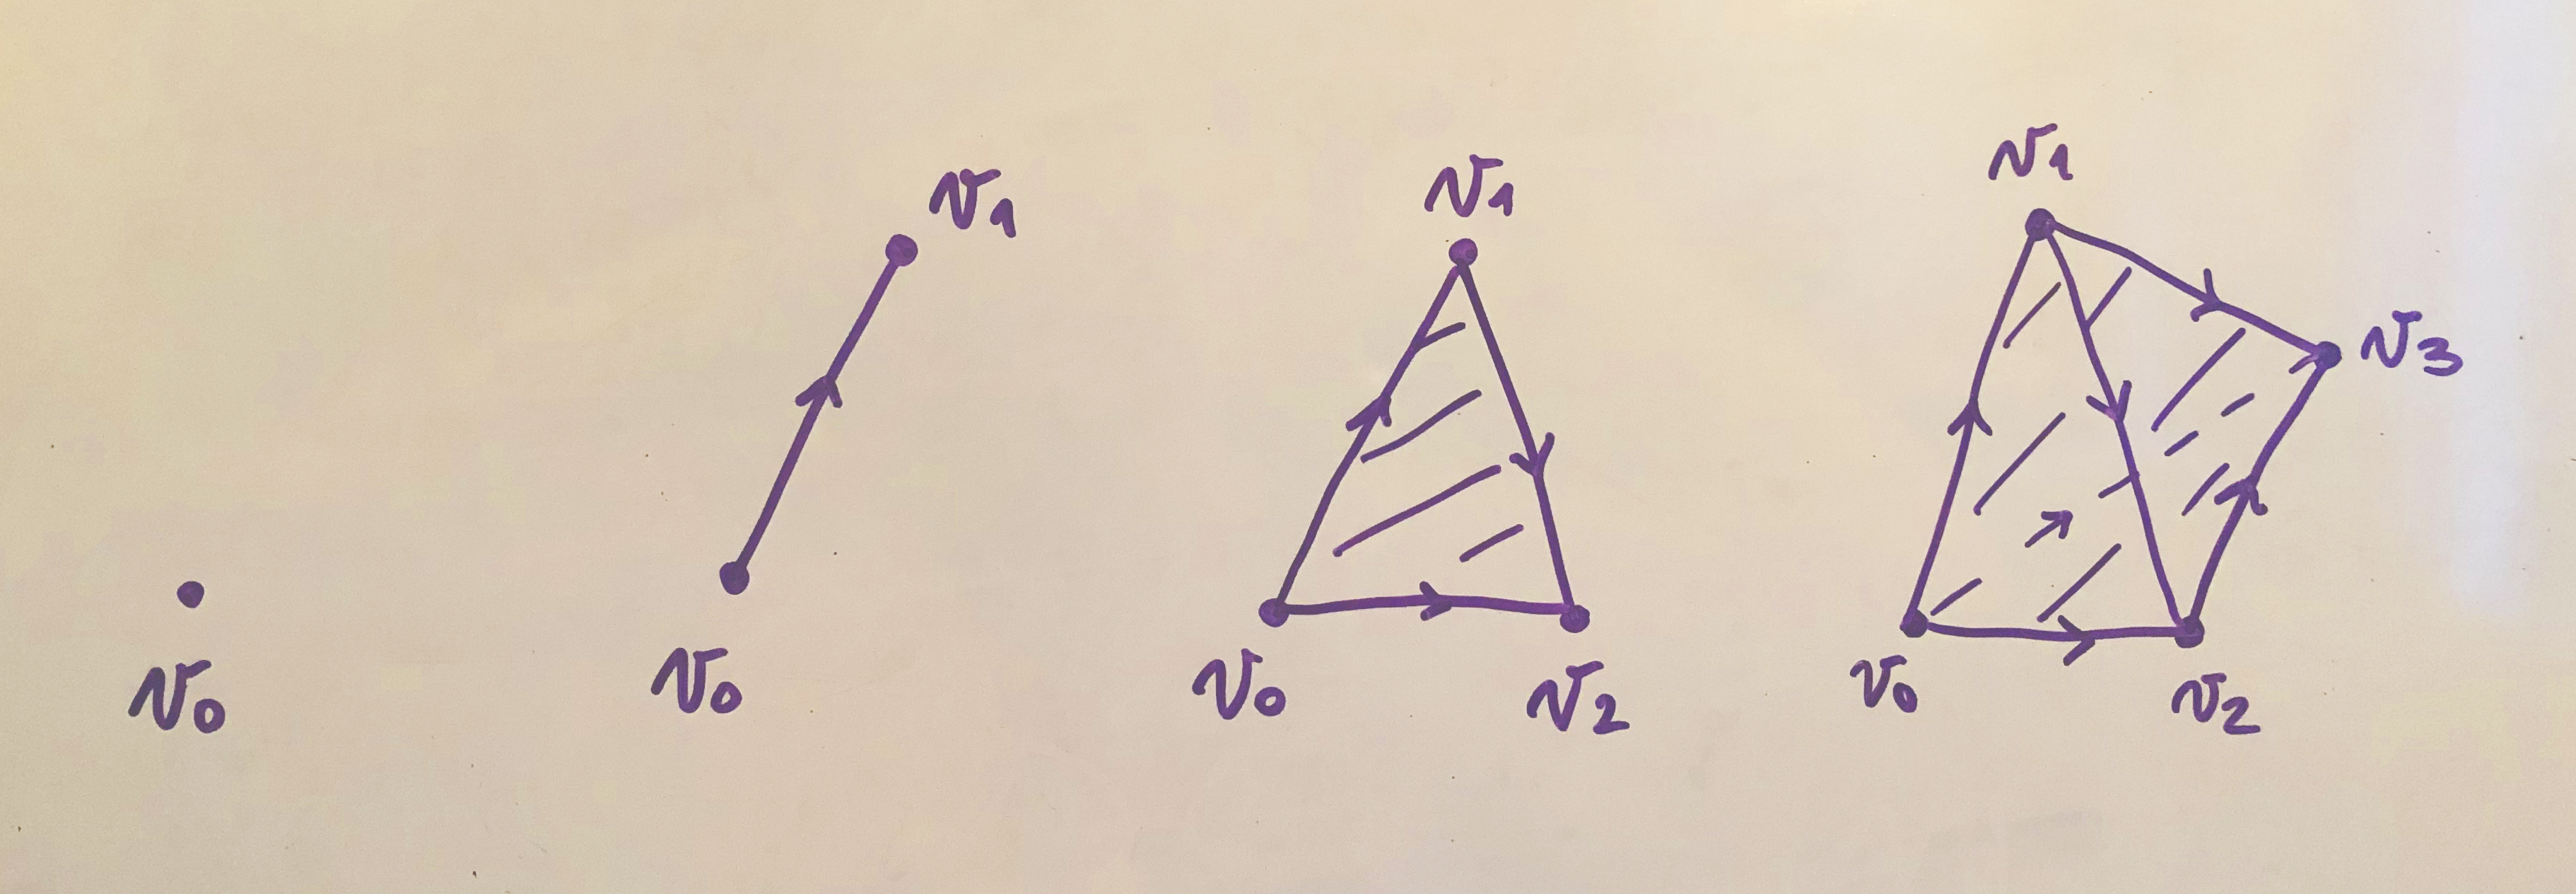
\includegraphics[width=0.5\linewidth]{img mono/simplices.png}
    \caption{$n$-símplices con las orientaciones de sus aristas, $n\in\{0,1,2,3\}$}
    \label{simplices}
\end{figure}

\comm{las imágenes no son finales, eventualmente las voy a hacer en digital}

\begin{df}
Llamaremos $n$-símplice estándar al conjunto $$\Delta^n := \Bigl\{(x_0,\dots,x_n)\in\R^{n+1} : x_i\geq 0\text{ para todo } i, \;\sum\limits_{i=0}^nx_i=1\Bigr\}$$
\end{df}

Los vértices de este $n$-símplice son los que conforman la base canónica de $\R^{n+1}$. Si notamos a estos puntos $e_1,\dots,e_{n+1}$, otra forma de escribir este conjunto es $$\Delta^n=[e_1,\dots,e_{n+1}] \subset \R^{n+1}$$\br

Para $n=2$, el $2$-símplice estándar $\Delta^2$ es el triángulo en $\R^3$ con vértices $(1,0,0)$, $(0,1,0)$ y $ (0,0,1)$. Con $n=1$, el $1$-símplice estándar es el segmento que va de $(1,0)$ a $(0,1)$ en $\R^2$. Esto se muestra en la imagen \ref{estandar}.\br

\begin{figure}[h!]
    \centering
    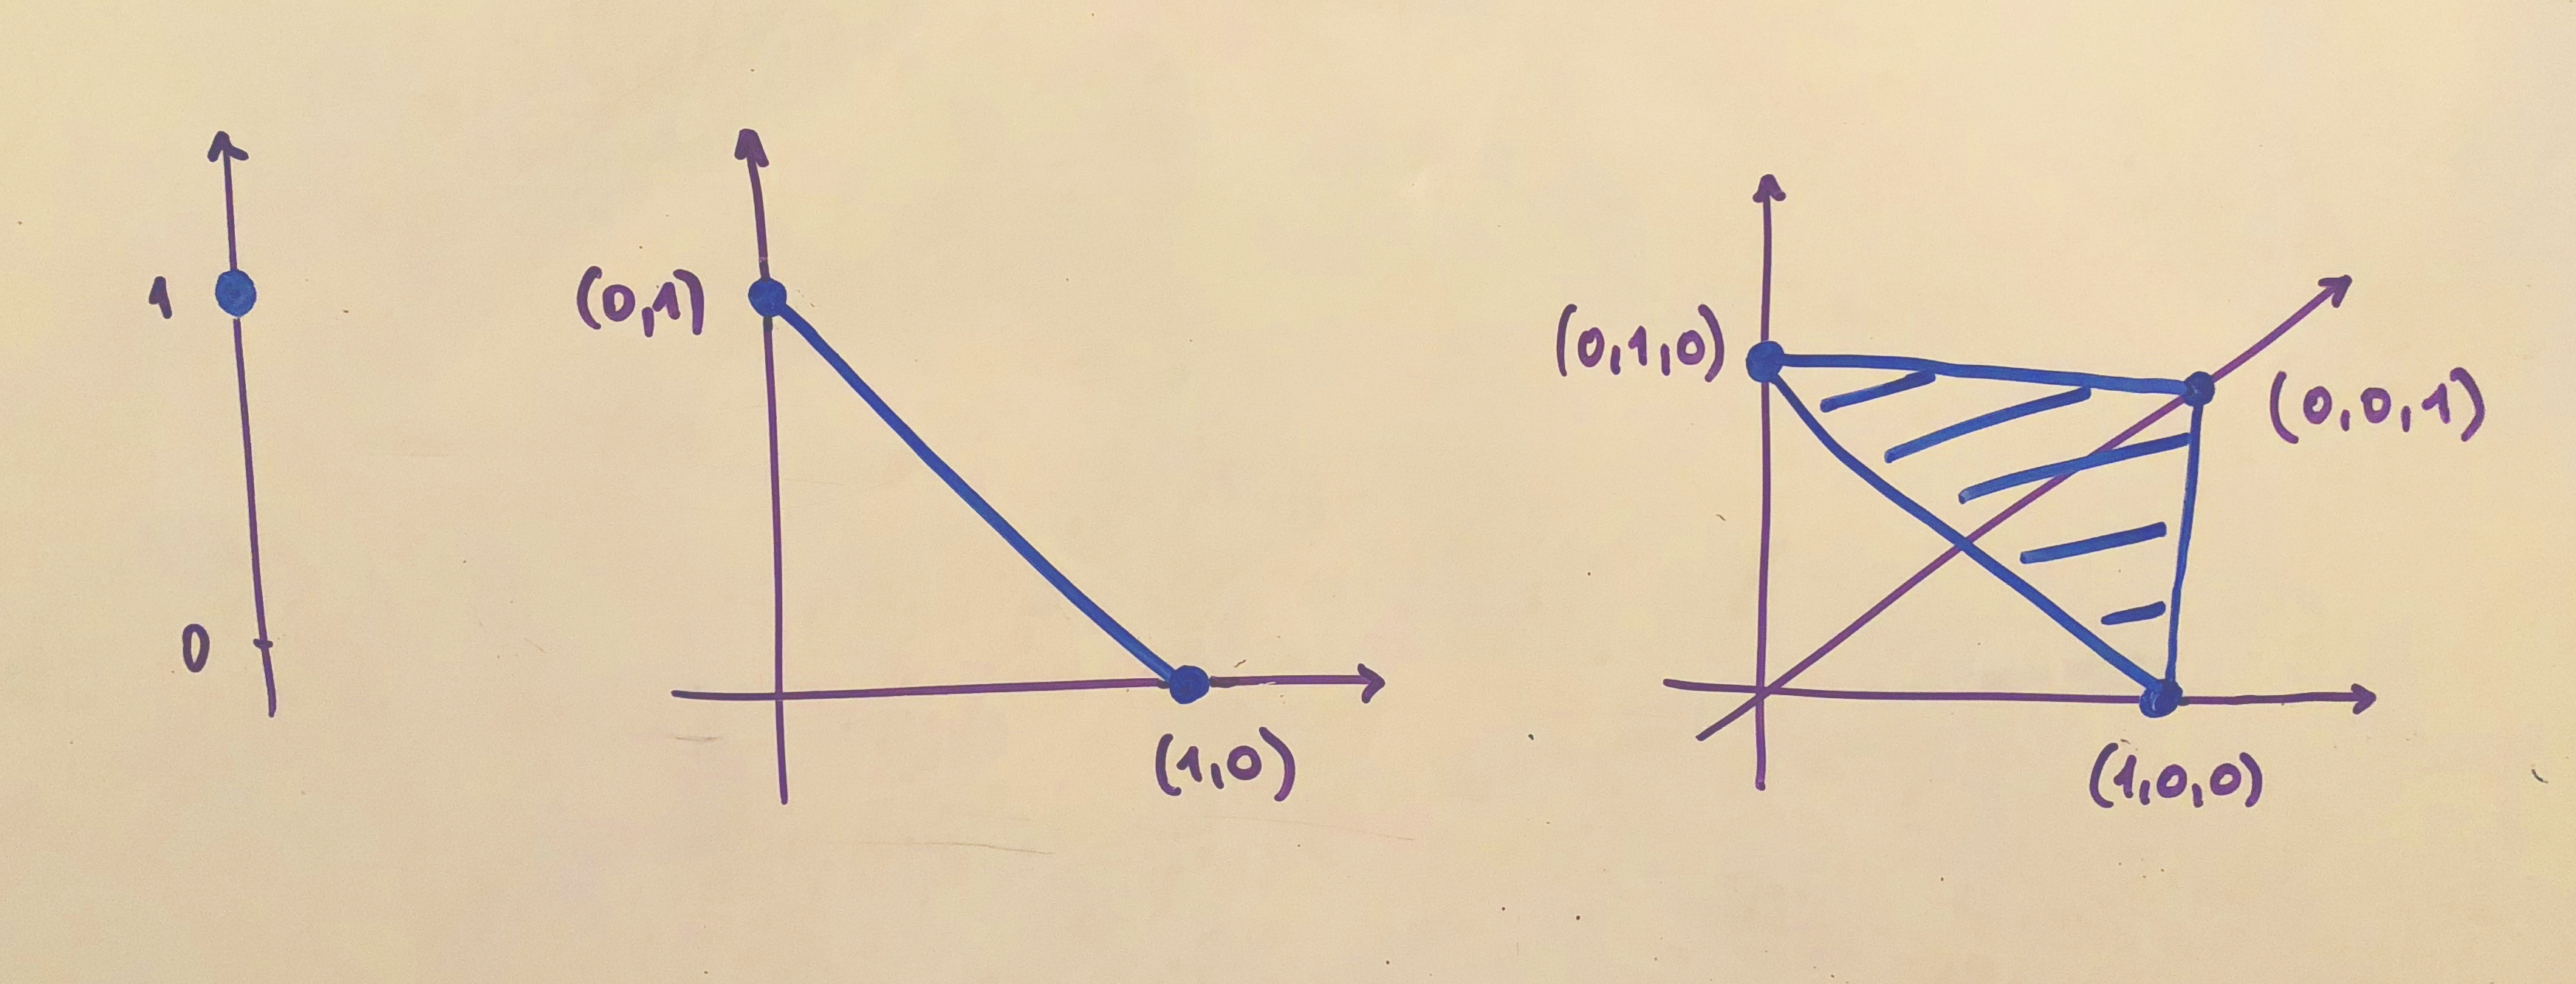
\includegraphics[width=0.5\linewidth]{img mono/simplices estandar.png}
    \caption{$n$-símplices estándar, $n\in\{0,1,2\}$}
    \label{estandar}
\end{figure}

\begin{df}
Dado un $n$-símplice $[v_0,\dots,v_n]$,  la función $h:\Delta^n\to [v_0,\dots,v_n]$ dada por $$h(x_0,\dots,x_n)=\sum\limits_{i=0}^n x_i v_i$$ es un homeomorfismo lineal que preserva el orden de las aristas. Llamaremos a esta función el homeomorfismo canónico.
\end{df}\br

La función $h$ es lineal y manda los elementos $e_0,\dots,e_n$ de la base canónica de $\R^{n+1}$ a $v_0,\dots, v_n$ respectivamente, por lo tanto su imagen es el $n$-símplice $[v_0,\dots,v_n]$ y el orden de las aristas se mantiene.\br

Antes de entrar en la definición de homología singular, vamos a definir la homología simplicial, que nos va a dar una imagen de las intuiciones que en la homología singular se ven más ofuscadas a cambio de obtener una teoría menos rígida y más limpia para trabajar.  \comm{cambiar este párrafo}\br

Para empezar, vamos a definir lo que será una estructura de $\Delta$-complejo para un espacio topológico cualquiera. Esto va a ser el análogo en dimensión $n$ de triangular nuestro espacio con $2$-símplices.\br


\begin{df}
    Una estructura de $\Delta$-complejo para un espacio topológico $X$ es una familia de funciones continuas $\sigma_\alpha:\Delta^{n_\alpha}\to X$ que cumplen:\br

    \begin{enumerate}
        \item Las $\sigma_\alpha$ son inyectivas al restringirlas a $Int(\Delta^{n_\alpha})$, y dado cualquier $x\in X$, existe algún $\alpha$ tal que $x$ está en la imagen de $Int(\Delta^{n_\alpha})$ por $\sigma_\alpha$.
        
        \item Si restringimos cualquier $\sigma_\alpha$ a una cara de $\Delta^{n_\alpha}$, esa restricción va a ser equivalente a otro mapa de la familia $\sigma_\beta:\Delta^{n_\alpha-1}\to X$, identificando la cara de $\Delta^{n_\alpha}$ con $\Delta^{n_\alpha-1}$ mediante el homeomorfismo canónico.

        \item Un conjunto $U\subset X$ es abierto $\iff$ $\sigma_\alpha^{-1}(U)$ es abierto para todo $\alpha$.
    \end{enumerate}
\end{df}\br

Las condiciones $(1)$ y $(3)$ nos dicen que las funciones $\sigma_\alpha$ restrictas a $Int(\Delta^{n_\alpha})$ son homeomorfismos sobre su imagen.\br

En el punto $(2)$, la equivalencia es en el siguiente sentido: \br

Dada $\sigma_\alpha:\Delta^{n_\alpha}\to X$, notamos $\hat{\Delta}^{n_\alpha}$ a una cara de $\Delta^{n_\alpha}$. Consideramos $h:\Delta^{n_\alpha -1}\to\hat{\Delta}^{n_\alpha}$ el homeomorfismo canónico que manda el $\{n_\alpha -1\}$-símplice estándar a $\hat{\Delta}^{n_\alpha}$. Lo que nos dice este punto es que existe una función $\sigma_\beta:\Delta^{n_\alpha -1}\to X$ en la familia que cumple $\sigma_\beta=\sigma_\alpha\circ h$. Decimos entonces que $\sigma_\alpha |_{\hat{\Delta}^{n_\alpha}}$ es equivalente a $\sigma_\beta$ y lo notaremos $\sigma_\alpha |_{\hat{\Delta}^{n_\alpha}}\simeq\sigma_\beta$.\br

Si por cada elemento $\sigma_\alpha:\Delta^{n_\alpha}\to X$ proveniente de la estructura de $\Delta$-complejo de $X$ consideramos un $n_\alpha$-símplice $\Delta^{n_\alpha}_\alpha$, entonces $X$ es el espacio obtenido al tomar el cociente de $x\sim h(x)$ para todas las $h:\Delta^{n_\alpha -1}\to \hat{\Delta}^{n_\alpha}_\alpha$ definidas como en el párrafo anterior. Algunos ejemplos se muestran en la imagen \ref{cocientes}.\br

\begin{figure}[h!]
    \centering
    \begin{subfigure}[]{0.4\linewidth}
        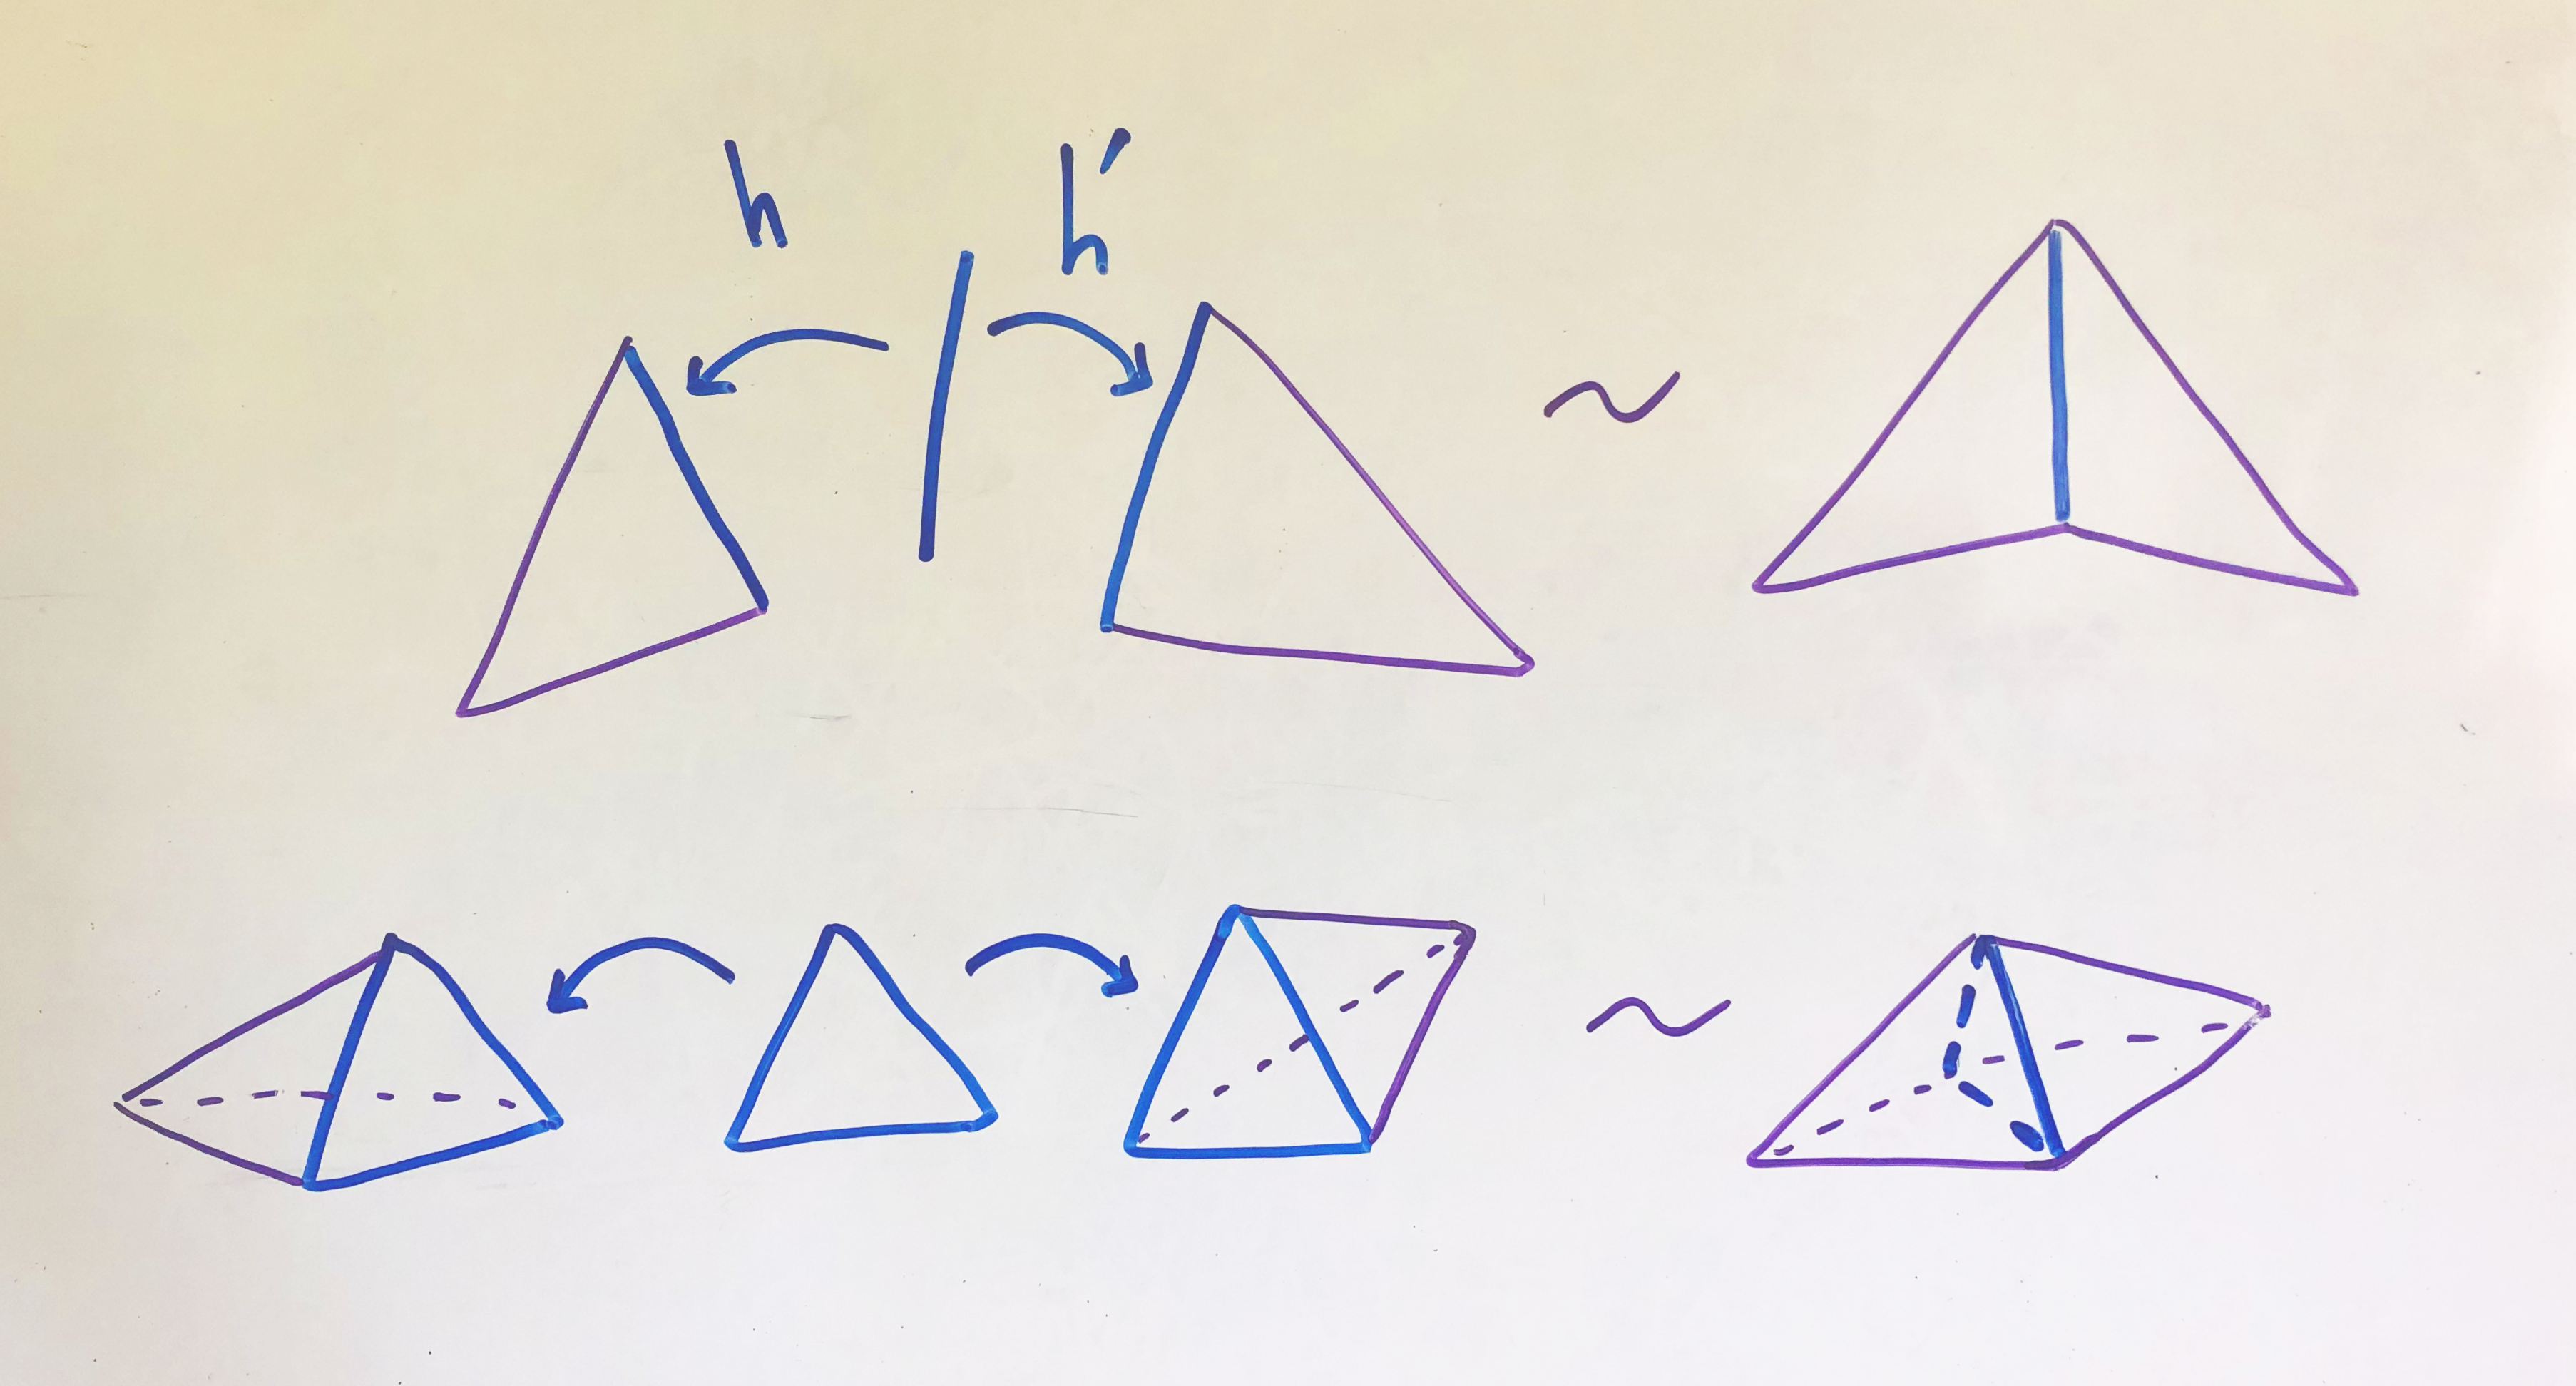
\includegraphics[width=\linewidth]{img mono/cociente.png}
    \end{subfigure}
    \begin{subfigure}[]{0.4\linewidth}
        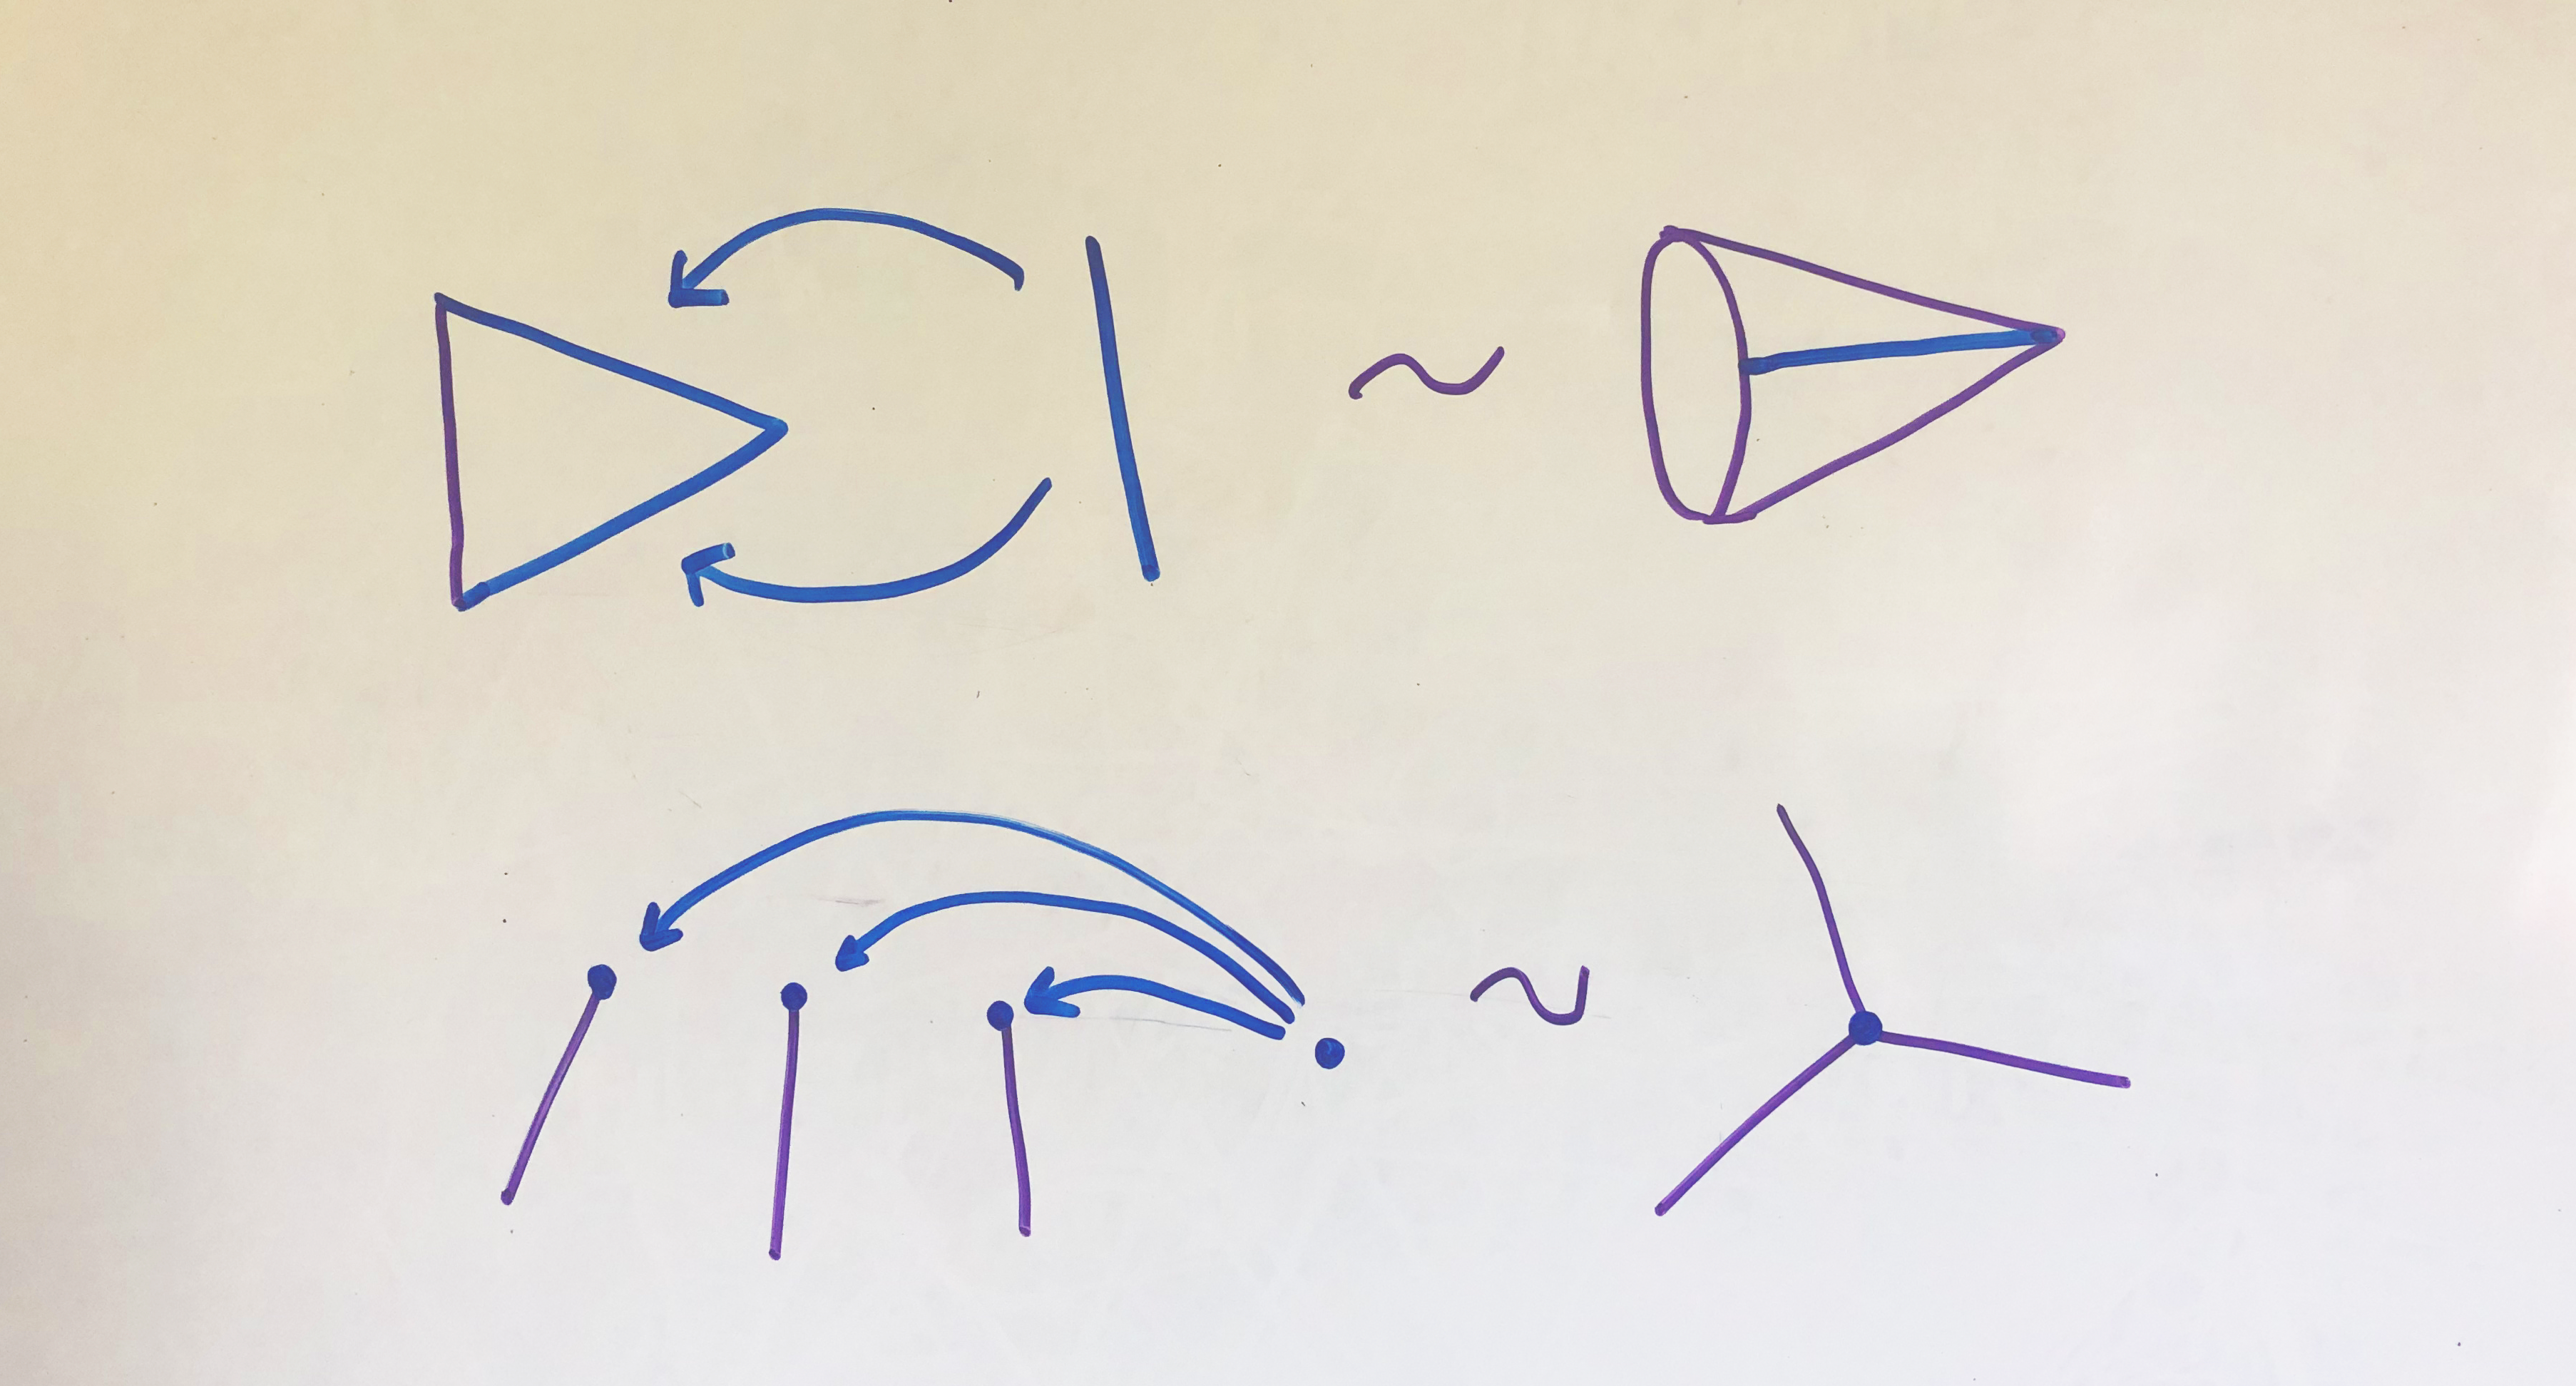
\includegraphics[width=\linewidth]{img mono/cociente2.png}
    \end{subfigure}
    \caption{Cocientes de símplices}
    \label{cocientes}
\end{figure}

\comm{me gustaría mejorar cómo está redactado pero no quiero abusar de los subíndices, porque sería una $h$ por cada cara de cada símplice}\br

%\begin{obs}
%Cualquier espacio con una estructura de $\Delta$-complejo va a ser Hausdorff, 
%\end{obs}

%\comm{capaz decir algo más acá y poner una imagen, obs sobre hff}

\begin{df}
    Dada una estructura de $\Delta$-complejo para un espacio $X$, definimos $\dx$ como el grupo abeliano libre generado por los $\{\sigma_\alpha:\Delta^{n_\alpha}\to X \; | \; n_\alpha=n\}$. Es decir, los elementos de $\dx$, a los que llamaremos $n$-cadenas, son sumas formales finitas $\sum_{i=1}^{N} k_i\sigma_i$, con $k_i\in\N$.
\end{df}

Nuestro objetivo ahora será definir un homomorfismo de grupos $\partial_n:\dx\to\ddx$ al que llamaremos mapa borde. Para motivar la definición primero nos enfocaremos en dimensiones $2$ y $3$, consideramos entonces las caras de $\Delta^2$ y $\Delta^3$.\br

En la imagen \ref{mal orientado} se muestra la orientación usual de las caras de cada uno de estos símplices, derivada del orden en sus vértices.\br

\begin{figure}[h!]
    \centering
    \begin{subfigure}[]{0.2\linewidth}
        \includegraphics[width=\linewidth]{img mono/norient2.png}
        \caption{$[v_1,v_2]$, $[v_0,v_2]$ y $[v_0,v_1]$}
    \end{subfigure}
    \hspace{2cm}
    \begin{subfigure}[]{0.2\linewidth}
        \includegraphics[width=\linewidth]{img mono/norient4.png}
        \caption{$[v_1,v_2,v_3]$, $[v_0,v_2,v_3]$, $[v_0,v_1,v_3]$ y $[v_0,v_1,v_2]$}
    \end{subfigure}
    \caption{Orientación usual}
    \label{mal orientado}
\end{figure}

A continuación, en la imagen \ref{bien orientados} ilustramos cómo quedan orientadas las caras si revertimos la orientación de los $[v_0,\dots,\hat{v_i},\dots,v_n]$ con $i$ impar.\br

\begin{figure}[h!]
    \centering
    \begin{subfigure}[]{0.2\linewidth}
        \includegraphics[width=\linewidth]{img mono/borient2.png}
        \caption{$[v_1,v_2]$, $-[v_0,v_2]$ y $[v_0,v_1]$}
    \end{subfigure}
    \hspace{2cm}
    \begin{subfigure}[]{0.2\linewidth}
        \includegraphics[width=\linewidth]{img mono/borient4.png}
        \caption{$[v_1,v_2,v_3]$, $-[v_0,v_2,v_3]$, $[v_0,v_1,v_3]$ y $-[v_0,v_1,v_2]$}
    \end{subfigure}
    \caption{Orientación obtenida al intercalar los signos}
    \label{bien orientados}
\end{figure}

\comm{sé que el formato de las imágenes está muy feo acá, en el futuro acomodaré todo eso cuando agregue las imágenes finales}

La idea entonces es que para obtener una orientación coherente y homogénea en las caras de nuestro símplice, vamos a intercalar la orientación usual de las caras con la orientación revertida. \br

\begin{df}

Procedemos ahora a definir el homomorfismo $\partial_n:\dx\to\ddx$. Para esto, fijamos su valor en los generadores de $\dx$, es decir, las funciones $\displaystyle{\sigma_\alpha:\Delta^n\to X}$. Notando $\Delta^n=[v_0,\dots,v_n]$, definimos $$\partial_n(\sigma_\alpha):=\sum\limits_{i=0}^{n}(-1)^i \sigma_\alpha|_{[v_0,\dots,\hat{v_i},\dots v_n]}$$ 

\end{df}

Definir el homomorfismo de esta manera lo dota de la siguiente propiedad, que será esencial para el desarrollo de la teoría:

\begin{lema}
La composición $\partial_{n-1}\circ\partial_n :\dx\to \Delta_{n-2}(X)$ es cero.
\end{lema}

\begin{dem}
Veamos que vale para $\sigma:\Delta^n\to X$ perteneciente a los generadores de $\dx$. La composición queda de la siguiente manera: 

$$\partial_{n-1}\circ\partial_n(\sigma)=\sum\limits_{i=0}^n(-1)^i\bigg(\sum\limits_{j<i}^n (-1)^j\sigma|_{[v_0,\dots,\hat{v_j},\dots,\hat{v_i},\dots,v_n]} + \sum\limits_{j>i}^n (-1)^{j-1}\sigma|_{[v_0,\dots,\hat{v_i},\dots,\hat{v_j},\dots,v_n]}\bigg)$$

Es importante observar que en la última sumatoria obtenemos un $(-1)^{j-1}$ en vez de un $(-1)^j$. Esto se debe a que si $j>i$, entonces el vértice $v_j$ está en el lugar $j-1$ del $(n-1)$-símplice $[v_0,\dots,\hat{v_i},\dots,v_j,\dots, v_n]$. \br

Usando que $\partial_n$ y $\partial_{n-1}$ son homomorfismos de grupos podemos distribuir el $(-1)^i$ y obtener que cada término de la sumatoria es de la forma $(-1)^i(-1)^j\sigma|_{[v_0,\dots,\hat{v_j},\dots,\hat{v_i},\dots,v_n]}$ si $i>j$, o $(-1)^i(-1)^{j-1}\sigma|_{[v_0,\dots,\hat{v_i},\dots,\hat{v_j},\dots,v_n]}$ si $i<j$. Dos términos se cancelan al intercambiar $i$ por $j$ y por lo tanto concluimos $\partial_{n-1}\circ\partial_n(\sigma)=0$. $\square$\br

\end{dem}

\begin{df}
    
Obtuvimos una familia de homomorfismos $\partial_n$ entre grupos abelianos libres $\dx$ que cumplen $\partial_{n-1}\circ\;\partial_n= 0$. Agregando un último elemento $\partial_0:\Delta_0(X)\to 0$ que definimos trivialmente, tenemos 

$$\dots\rightarrow \Delta_{n+1}(X)\xrightarrow{\partial_{n+1}}\dx\xrightarrow{\partial_n}\ddx\rightarrow\dots\rightarrow\Delta_{1}(X)\xrightarrow{\partial_1}\Delta_{0}(X)\xrightarrow{\partial_0} 0$$\br

Llamamos a una familia como esta un complejo de cadenas.

\end{df}\br

Otra forma de describir la propiedad $\partial_{n-1}\circ\;\partial_n=0$ es decir que $\im(\partial_{n+1})\subset\Ker(\partial_n)$, con esto vamos a definir los grupos de homología del complejo de cadenas.\br

\begin{df}

Definimos el $n$-ésimo grupo de homología simplicial del complejo de cadenas como el cociente $$H_n^{\Delta}(X):=\Ker(\partial_n)/\im(\partial_{n+1})$$\br

Llamamos ciclos a los elementos de $\Ker(\partial_n)$ y bordes a los de $\im(\partial_{n+1})$. Los elementos de $H_n^{\Delta}(X)$ serán nuestras clases de homología simplicial.\br 

Diremos que dos ciclos que pertenecen a la misma clase de homología simplicial son ciclos homólogos. Dos ciclos $\sum_{i=0}^N k_i\sigma_i$ y $\sum_{i=0}^M k'_i\sigma'_i$ de esta manera cumplirán que su diferencia $\sum_{i=0}^N k_i\sigma_i - \sum_{i=0}^M k'_i\sigma'_i$ es un borde.\br

\end{df}

\comm{En algún momento debería hacer una observación sobre por qué uso $\Delta$-complejos en vez de complejos simpliciales, que son los que dan el nombre a la homología simplicial. La verdad es que lo hago así porque hatcher lo hace así, y él dice que lo hace así porque los $\Delta$-complejos son más generales y más fáciles de trabajar que los simpliciales, sin embargo la verdad es que todo esto lo podría haber hecho con complejos simpliciales y no hubiera cambiado demasiado porque solo lo uso para introducir las intuiciones. O sea, \textit{mi} razón para hacerlo así es que hatcher lo hace así pero bueno debería decir algo que no sea eso.}

A continuación nos enfocaremos en algunos ejemplos.

\begin{ex}
    Comenzemos con el ejemplo más sencillo. Tomamos $X = \{p\}$ un punto. Una estructura de $\Delta$-complejo para $X$ está dada por una única función $\{\sigma_0:\Delta^0\to X\}$. \br
    
    Los grupos $\Delta_n(X)$ son $0$ salvo para $n=0$, en ese caso se tiene $\Delta_0(X)=\langle\sigma_0\rangle\simeq\Z$. Por esta razón, todos los homomorfismos $\partial_n:\dx\to\ddx$ son $0$, incluyendo $\partial_0:\Delta_0(X)\to 0$, que es $0$ por definición.\br

    Por lo tanto, en este caso tenemos $\im(\partial_n)=0$ para todo $n$, $\Ker(\partial_n)=0$ para todo $n\neq 0$, y $Ker(\partial_0)=\Delta_0(X)\simeq\Z$.\br

    Entonces $$H^{\Delta}_n(X)\simeq
    \begin{cases}
    0\text{ si } n\neq 0 \\
    \Z\text{ si } n=0
    \end{cases}$$
\end{ex}\br

\begin{ex}
Consideremos ahora $X=S^1$. Para darle una estructura de $\Delta$-complejo, vemos todo $S^1$ como una arista $e$ con un único vértice $v$ como se muestra en la imagen \ref{s1}. Nuestra estructura de $\Delta$-complejo para $X$ está dada por dos funciones $\sigma_0:\Delta^0\to X$ y $\sigma_1:\Delta^1\to X$. Si notamos $\Delta^1=[v_0,v_1]$ entonces $\im(\sigma_0)=\{v\}$, $\im(\sigma_1)=e$ y $\sigma_1|_{[v_0]}\simeq\sigma_1|_{[v_1]}\simeq\sigma_0$.\br

\begin{figure}[h!]
    \centering
    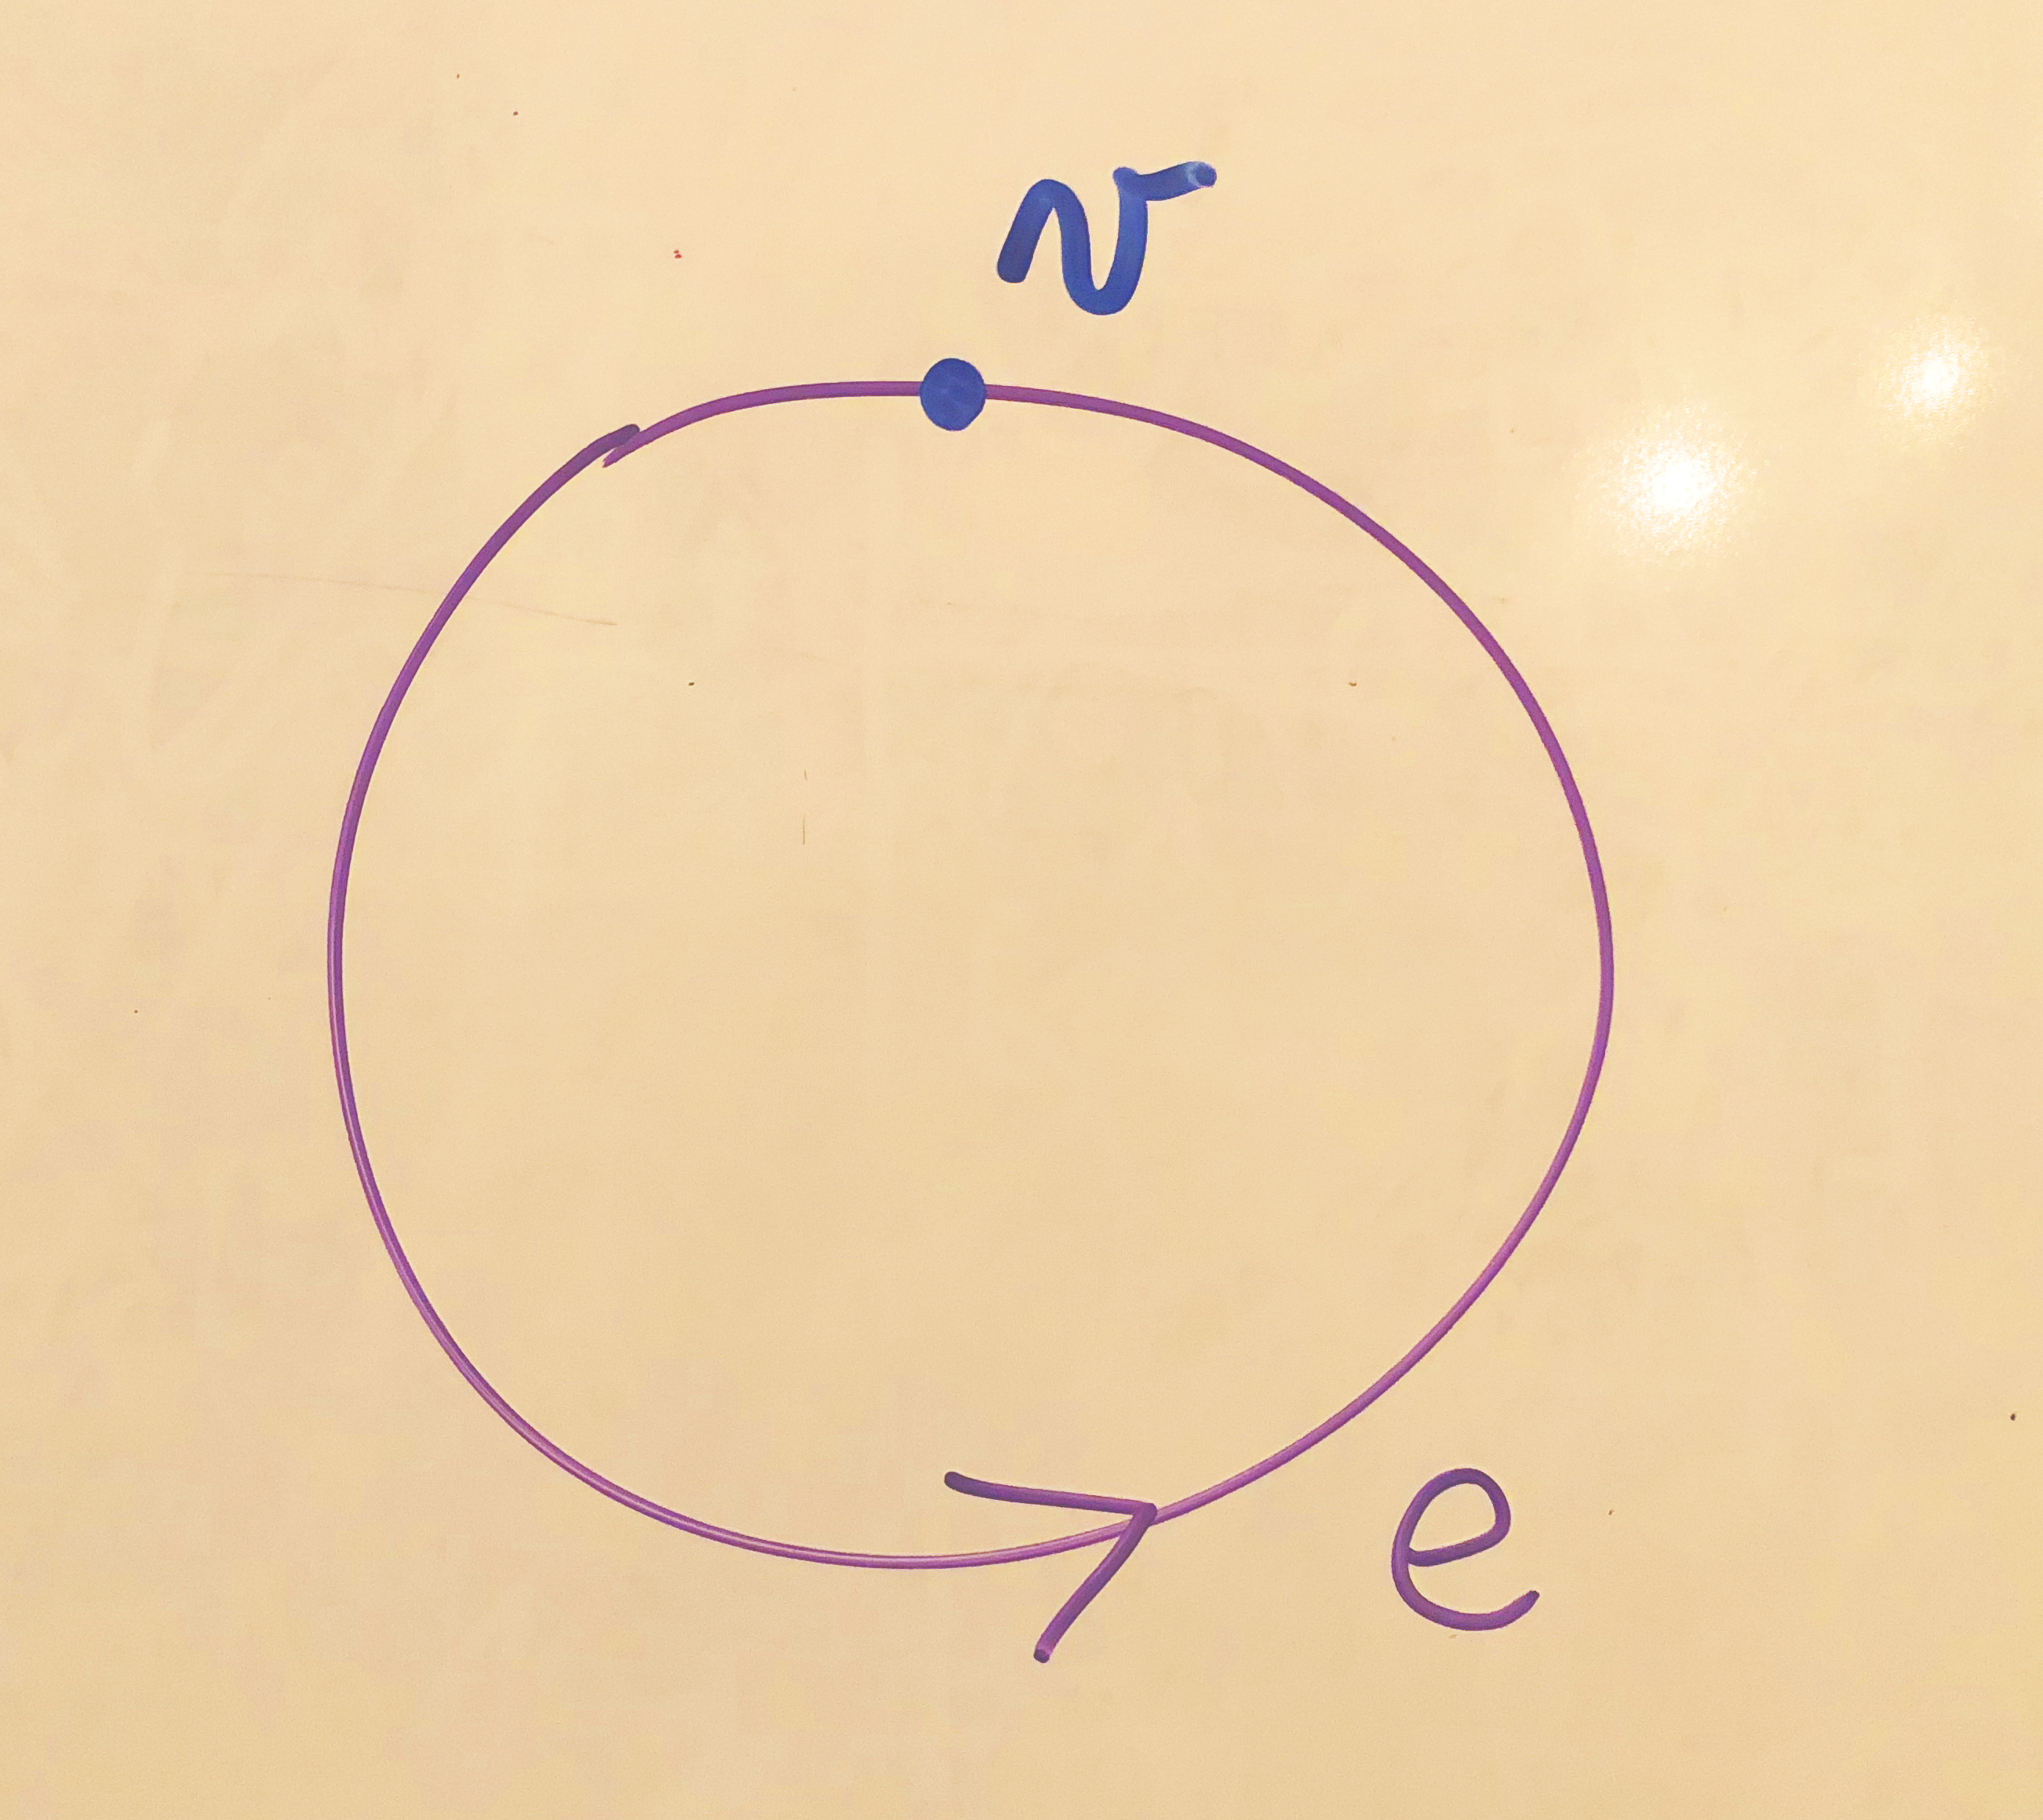
\includegraphics[width=0.3\linewidth]{img mono/s1.png}
    \caption{$S^1$}
    \label{s1}
\end{figure}

Los grupos $\dx$ son $0$ para todo $n\neq 0,1$. Para $n=1$ se tiene $\Delta_1(X)=\langle\sigma_1\rangle\simeq\Z$ y para $n=0$ se tiene $\Delta_0(X)=\langle\sigma_0\rangle\simeq\Z$.\br

Como $\sigma_1|_{[v_0]}\simeq\sigma_1|_{[v_1]}$, entonces $\partial_1(\sigma_1)=\sigma_1|_{[v_1]}-\sigma_1|_{[v_0]}=0$ y por lo tanto $\Ker(\sigma_1)=\Delta_1(X)$. Además sabemos que $\Delta_2(X)=0$ y por lo tanto $\im(\partial_2)=0$. Con esto obtenemos que $H^\Delta_1(X)\simeq\Z$.\br

En el caso de $H_0^\Delta(X)$, observamos que $\Ker(\partial_0)=\Delta_0(X)$ y $\im(\partial_1)=0$ por la misma razón que antes. Con esto obtenemos que $H^\Delta_0(X)\simeq\Z$.\br

Como $\dx=0$ para todo $n\neq 0,1$, concluimos que 

$$ H^{\Delta}_n(X)\simeq
    \begin{cases}
    0\text{ si } n\neq 0,1 \\
    \Z\text{ si } n\in\{0,1\}
    \end{cases} $$
\end{ex}

\begin{ex}

Sea $X=\T^2$, sabemos que podemos expresarlo como cociente de $[0,1]^2$. Para darle una estructura de $\Delta$-complejo, separamos $[0,1]$ en dos triángulos como se ve en la imagen \ref{toro}, que llamamos $U$ y $L$. Los bordes de estos triángulos, después de pasar por el cociente, serán nuestras tres aristas $a,b$ y $c$, que comparten un único vértice $v$. 

\begin{figure}[h!]
    \centering
    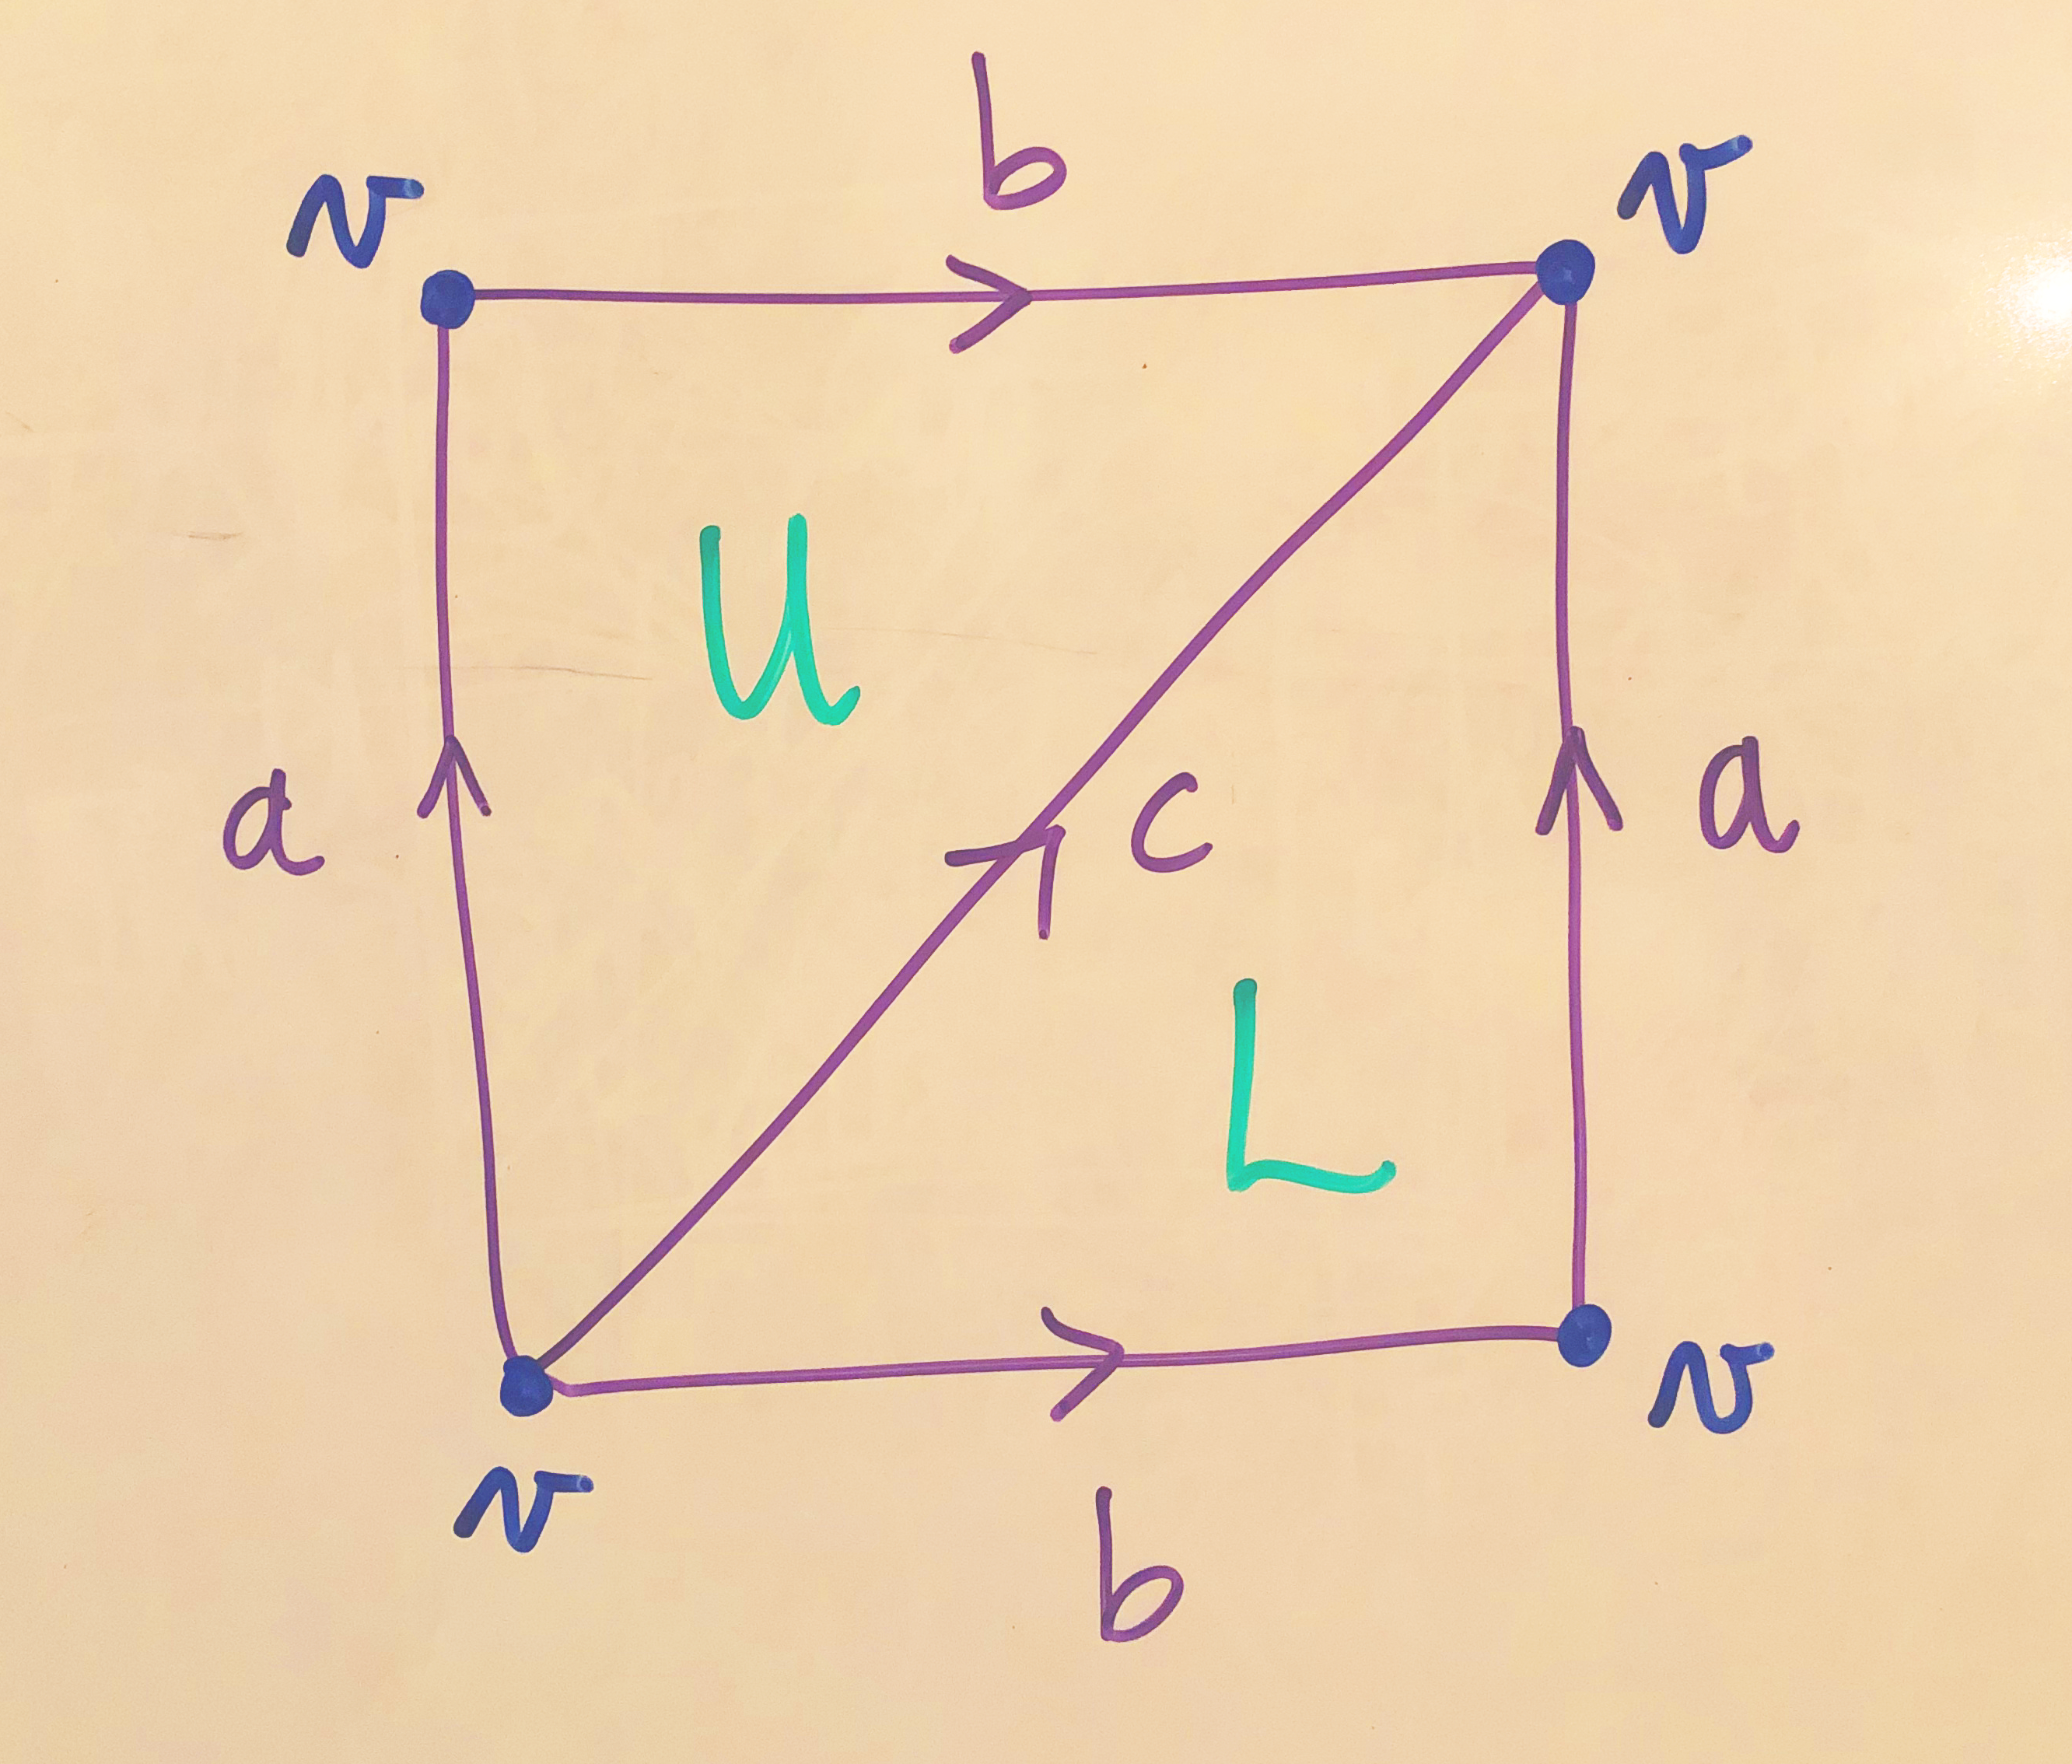
\includegraphics[width=0.3\linewidth]{img mono/toro.png}
    \caption{$\T^2$}
    \label{toro}
\end{figure}

Una estructura de $\Delta$-complejo para $X$ está dada por $\{\sigma_2^1,\sigma_2^2,\sigma_1^1,\sigma_1^2,\sigma_1^3,\sigma_0\}$, con 

$$\begin{cases}
    \sigma_2^1:\Delta^2\to U\\
    \sigma_2^2:\Delta^2\to L\\
    \sigma_1^1:\Delta^1\to a\\
\end{cases}\hspace{1cm}
\begin{cases}
    \sigma_1^2:\Delta^1\to b\\
    \sigma_1^3:\Delta^1\to c\\
    \sigma_0:\Delta^0\to \{v\}\\
\end{cases}$$

Si notamos $\Delta^2=[v_0,v_1,v_2]$, $\Delta^1=[w_0,w_1]$, entonces se cumplen las relaciones \br
$$\begin{cases}
    \sigma_2^1|_{[\hat{v_0},v_1,v_2]}\simeq\sigma_1^2\\
    \sigma_2^1|_{[v_0,\hat{v_1},v_2]}\simeq\sigma_1^3\\
    \sigma_2^1|_{[v_0,v_1,\hat{v_2}]}\simeq\sigma_1^1
\end{cases}\hspace{0.5cm}
\begin{cases}
    \sigma_2^2|_{[\hat{v_0},v_1,v_2]}\simeq\sigma_1^1\\
    \sigma_2^2|_{[v_0,\hat{v_1},v_2]}\simeq\sigma_1^3\\
    \sigma_2^2|_{[v_0,v_1,\hat{v_2}]}\simeq\sigma_1^2
\end{cases}\hspace{0.5cm}
\begin{cases}
    \sigma_1^i|_{[\hat{w_0},w_1]}\simeq\sigma_0 \\
    \sigma_1^i|_{[w_0,\hat{w_1}]}\simeq\sigma_0 
\end{cases} \fall i\in\{1,2,3\}$$\br

Observar que estas relaciones están en parte determinadas por la orientación de los símplices, esto es parte de la rigidez que impone la teoría de los $\Delta$-complejos.\br

Tenemos entonces que $\dx=0$ para todo $n\neq 0,1,2$, $\Delta_2(X)=\langle\sigma_2^1, \sigma_2^2 \rangle\simeq\Z\oplus\Z$, $\Delta_1(X)=\langle\sigma_1^1,\sigma_1^2,\sigma_1^3\rangle\simeq\Z\oplus\Z\oplus\Z$, $\Delta_0(X)=\langle\sigma_0\rangle\simeq\Z$.\br

Estudiemos primero el caso de $\partial_2$. Se tiene $\partial_2(\sigma_2^1)=\sigma_1^2-\sigma_1^3+\sigma_1^1$. Haciendo un abuso de notación, podemos escribirlo como $\partial U=b-c+a$. De la misma manera, tenemos $\partial_2(\sigma_2^2)=\sigma_1^1-\sigma_1^3+\sigma_1^2$, que podemos escribir como $\partial L=a-c+b$. Por lo tanto, continuando con esta notación, la imagen de $\partial_2$ es el grupo abeliano libre generado por $a+b-c$. Por esto mismo también obtenemos que $\Ker(\partial_2)$ es el grupo abeliano libre generado por $U-L$, que es isomorfo a $\Z$.\br

Consideramos ahora $\partial_1$. Como $\sigma_1^i|_{[\hat{w_0},w_1]}\simeq\sigma_0\simeq\sigma_1^i|_{[w_0,\hat{w_1}]}$ para $i\in\{1,2,3\}$, tenemos que $\im(\partial_1)=0$ y $\Ker(\partial_1)=\Delta_1(X)$.\br

Como $\Delta_3(X)=0$ se cumple que $im(\partial_3)=\Ker(\partial_3)=0$. Para $\partial_0$ se cumple $\im(\partial_0)=0$ y $\Ker(\partial_0)=\Delta_1(X)$ trivialmente.\br

Con esto, continuando con el abuso de notación tenemos que 
\begin{align*}
        &H^\Delta_2(X)=\Ker(\partial_2)/\im(\partial_3)\simeq\Z \\
        &H^\Delta_1(X)=\Ker(\partial_1)/\im(\partial_2)=\langle a,b,c \;|\; a+b-c=0\rangle\simeq \Z\oplus\Z \\
        &H^\Delta_0(X)=\Ker(\partial_0)/\im(\partial_1)\simeq\Z
\end{align*}

y todos los demás $H^\Delta_n(X)$ se anulan.

\comm{es posible que este ejemplo sea mucha notación}
\end{ex}
\comm{me gustaría poner algunos ejemplos más, me gustaría pegar un par de 2-símplices para mostrar cómo el borde queda solo la parte de afuera y todo lo de adentro se cancela}

\begin{obs}
    Recordar que llamamos bordes a los elementos de $\im(\partial_n)$ y ciclos a los de $\Ker(\partial_n)$. La idea detrás de estos nombres puede comenzar a aclararse observando el caso de $H^\Delta_1(X)$ para un espacio $X$ cualquiera.\br
    
    Si notamos $\Delta^1=[v_0,v_1]$ y tomamos $\sigma_i:\Delta^1\to X$ provenientes de la estructura de $\Delta$-complejo de $X$ entonces un elemento de $\Ker(\partial_1)$ es una suma formal $\sum k_i\sigma_i$ con $\sum k_i\sigma_i|_{[\hat{v_0},v_1]} - \sum k_i\sigma_i|_{[v_0,\hat{v_1}]}=0$. Un elemento de esta manera debe cumplir que cada vértice tiene el mismo número de aristas entrantes y salientes. Al ver $X$ como cociente de símplices, esto se traduce en la noción de que las imágenes de las $\sigma_i$ forman curvas cerradas.\br

    Un elemento de $\im(\partial_2)$ es también un elemento de $Ker(\partial_1)$, y por lo tanto su imagen pasada por el cociente también es unión de curvas cerradas. Sin embargo, a diferencia de los elementos de $\Ker(\partial_1)$, estas curvas cerradas necesariamente son el borde de algún $\Delta$-complejo de dimensión 2, por ejemplo de un disco.\br

    Lo que logra $H_1^\Delta(X)$ es distinguir las curvas cerradas contractibles de las no contractibles en $X$. Es decir, distingue las curvas cerradas que son borde de algún complejo de dimensión 2 de las que bordean un "agujero" en $X$. Dicho usando la nomeclatura de ciclos y bordes, los elementos relevantes para $H_1^\Delta$ son los ciclos que no son borde de ningun $2$-complejo.\br
\end{obs}

Finalmente, tiene sentido plantearnos la pregunta: Dadas dos estructuras de $\Delta$-complejo para un mismo espacio $X$, son los grupos $H^\Delta_n(X)$ isomorfos? \br

La respuesta es que si, y veremos la prueba en el siguiente capítulo.


\chapter{Homología singular}

El objetivo de este capítulo será definir los grupos de homología singular de un espacio topológico $X$. Esta definición es muy similar a la vista en el capítulo anterior, con la notoria diferencia de que en vez de considerar una estructura de $\Delta$-complejo para $X$, directamente tomamos el cociente en la familia de todas las funciones $\sigma:\Delta^n\to X$.

\begin{df}
    Un $n$-símplice singular es una función continua $\sigma:\Delta^n\to X$.
\end{df}

El nombre "singular" hace referencia a que $\sigma$ no tiene por qué ser inyectiva, por lo tanto no necesariamente es un encaje. Esto significa que la imagen de $\sigma$ puede tener singularidades, es decir, puntos de autointersección. \br

\duda{acá solo dice que puede tener "sigularidades" pero no explica, yo lo interpreto así, como puntos de autointersección, pero capaz hay algo más que se me está pasando?}

\begin{df}
    Llamaremos complejo de $n$-cadenas singulares, que notaremos $C_n(X)$, al grupo abeliano libre que tiene como base a los elementos de la familia de funciones $\{\sigma:\Delta^n\to X \;\vert\; \sigma \text{ continua}\}$. \br

    Es decir, los elementos de $C_n(X)$, a los que llamaremos $n$-cadenas singulares, serán sumas formales finitas $\sum_{i=1}^k n_i\sigma_i$, con $n_i\in\Z$, y $\sigma_i:\Delta^n\to X$.
\end{df}

Comparados con su equivalente $\Delta^n(X)$ del capítulo anterior, los complejos de $n$-cadenas singulares $C_n(X)$ tienen un cardinal mucho más grande, y en la mayoría de los casos serán  grupos no numerables. \br

\begin{df}
    Definimos un mapa borde $\partial_n:\Ch\to\ch$ dado por $$\partial_n(\sigma):= \sum\limits_{i=0}^{n}(-1)^i \sigma |_{[v_0,\dots,\hat{v_i},\dots,v_n]}$$ 
    Donde estamos notando $\Delta^n$ como $[v_0,\dots,v_n]$ e identificando $[v_0,\dots,\hat{v_i},\dots,v_n]$ con $\Delta_{n-1}$ mediante el homeomorfismo canónico.
\end{df}

En algunos casos simplemente usaremos $\partial$ para notar este mapa.\br

Exactamente de la misma forma que en el capítulo anterior, obtenemos que la composición $\partial_{n-1}\circ\partial_n :C_{n}(X)\to C_{n-2}(X)$ es cero. Por lo tanto tenemos $\im(\partial_{n-1})\subset\Ker(\partial_{n})$ y podemos definir los grupos de homología singular.\br

\begin{df}
Definimos el $n$-ésimo grupo de homología singular del complejo de cadenas como el cociente $$H_n(X):=\Ker(\partial_n)/\im(\partial_{n+1})$$\br

De la misma forma que antes llamaremos ciclos a los elementos de $\Ker(\partial_n)$, bordes a los de $\im(\partial_{n+1})$ y los elementos de $H_n(X)$ serán nuestras clases de homología singular.\br 
\end{df}

Con esta definición, obtenemos trivialmente un resultado importante para la teoría.

\begin{prop}
Si $X$, $Y$ son homeomorfos, entonces $H(X)=H(Y)$
\end{prop}
\begin{proof}
Sean $h:X\to Y$ homeomorfismo. Dada $sigma:\Delta^n\to X$ continua, consideramos su composición $h\circ\sigma$
\end{proof}









\chapter{Contraejemplos a la generalización de Jordan-Schönflies}



\chapter{Límites inversos y atractores de sistemas dinámicos}



\end{document}